\chapter{ Luminometer system and calibration description}

%%%%Introduction%%%%%%%%%%%%%%%%%%%%5

A total of seven systems are used for measuring luminosity at CMS, being the PCC one of them. 




%%%%%%%%%%%%%%%%%%%%%%%%%%%%%%%%%%%%%%%%%%%%%%%%%%%%%%%%%%%%%%%%%%%%%%%%%%%%%%%%%%%%%%%%%
\section{Pixel Clusters and the PCC method}

Luminosity measurements at CMS are provided by the several luminometers in the detector.
Each luminometer measures the event rate by reading out a specific quantity of objects observed by the detector, These can be for example clusters, coincidences or tracks. For the TEPX luminometers these objects are pixel clusters and coincidences, using the pixel cluster counting (PCC) method to provide offline luminosity measurements. This method was one of the main source of luminosity measurements for CMS, during the 2016-2018 data taking period, and it is expected to be the same for the Phase-2 upgrade.\\
The clustering algorithm is very complex, but striping it down to the most simple example: the algorithm considers a cluster of pixels only if two hits, or more,  activate neighboring pixels horizontally, vertically or diagonally, within the same module. Figure\ref{pixclust} shows an example of this.
\begin{figure}[H]
\begin{minipage}[b]{0.5\linewidth}
\centering
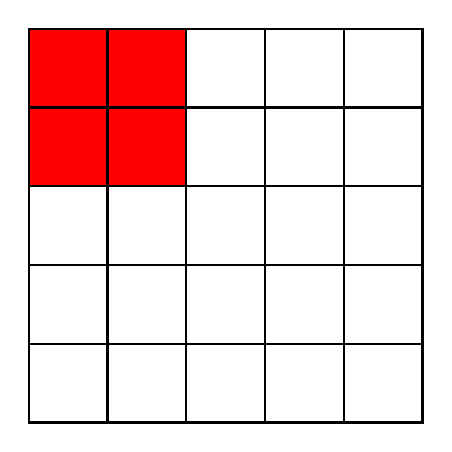
\begin{tikzpicture}
    [%%%%%%%%%%%%%%%%%%%%%%%%%%%%%%
        box/.style={rectangle,draw=black,thick, minimum size=1cm},
    ]%%%%%%%%%%%%%%%%%%%%%%%%%%%%%%

\foreach \x in {0,1,...,4}{
    \foreach \y in {0,1,...,4}
        \node[box] at (\x,\y){};
}

\node[box,fill=red  ] at (1,4){};  
\node[box,fill=red ] at (0,4){};  
\node[box,fill=red ] at (0,3){}; 
\node[box,fill=red  ] at (1,3){};
\end{tikzpicture}
\end{minipage}
\begin{minipage}[b]{0.5\linewidth}
\centering
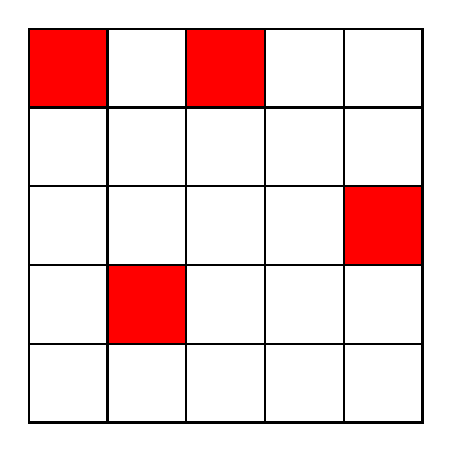
\begin{tikzpicture}
    [%%%%%%%%%%%%%%%%%%%%%%%%%%%%%%
        box/.style={rectangle,draw=black,thick, minimum size=1cm},
    ]%%%%%%%%%%%%%%%%%%%%%%%%%%%%%%

\foreach \x in {0,1,...,4}{
    \foreach \y in {0,1,...,4}
        \node[box] at (\x,\y){};
}
 
\node[box,fill=red  ] at (0,4){};  
\node[box,fill=red ] at (2,4){};  
\node[box,fill=red ] at (1,1){}; 
\node[box,fill=red ] at (4,2){}; 
\end{tikzpicture}
\end{minipage}
\caption[Pixel cluster selection algorithm]{The figure shows a representation of the pixel modules, \textit{left}: four hits (red) on four neighbouring pixels, these is considered a pixel cluster by the clustering algorithm. \textit{right}: the hits activate random pixel in the module, these will not be considered as a cluster by the clustering algorithm.}
\label{pixclust}
\end{figure}
A hit occurs when a charged particle passes through a silicon pixel, depositing an amount of energy in the pixel. The PCC method takes advantage of the high densities of pixels, and the relative low occupancy of the CMS tracker, to provide precise luminosity measurements, with good stable measurements over time. The number of pixel clusters activated, per bunch crossing, is a linear function of the number of proton-proton interactions per bunch crossing (pileup). During several zero-bias events, where the only requirement is that the bunches pass through one another on the interaction point, a mean number of pixel clusters, $\left\langle N_{\text {cluster }}\right\rangle
$,is activated:
\begin{equation}
\left\langle N_{\text {cluster }}\right\rangle\equiv\left\langle N_{\text {cluster/int}}\right\rangle\mu
\label{pcc}
\end{equation}
where $\left\langle N_{\text {cluster/int}}\right\rangle$ is the mean number of clusters activated per interaction and $\mu$ is the pileup. Using equation \ref{pileup} and \ref{pcc}, a calibration constant between the mean number of pixel cluster and the instantaneous luminosity can be defined:

\begin{equation}
    \left\langle N_{\text {cluster }}\right\rangle\equiv\frac{\sigma_{vis}}{f}\mathcal{L}_{ins}
\end{equation}
where the calibration constant, $\sigma_{vis}$, is   
\begin{equation}
    \sigma_{vis}=\sigma_{tot}\left\langle N_{\text {cluster/int}}\right\rangle
\end{equation}
The value of $\sigma_{vis}$ is determined using a van der Meer (vdM) scan, with 
\begin{equation}
    \sigma_{vis}= \frac{\left\langle N_{\text {cluster/vdM }}\right\rangle f }{\mathcal{L}_{ins/vdM}}
\end{equation}
where $\left\langle N_{\text {cluster/vdmM }}\right\rangle$ is the mean number of pixel cluster at the peak of the scan and $\mathcal{L}_{ins/vdM}$ is the instantaneous luminosity obtained in the scan \cite{CMS-PAS-LUM-12-001}.


%%%%%%%%%%%%%%%%%%%%%%%%%%%%%%%%%%%%%%%%%%%%%%%%%%%%%%%%%%%%%%%%%%%%%%%%%%%%%%%%%%%%%%%%%

\section{Calibration using the van der Meer method }
The calibration of the luminometrs is done by performing van der Meer scans, where the goal is to determine the calibration constant $\sigma_{\text {vis}}$.\\
In practice, the normalized bunch transverse distributions of each beam is not known, thus the overlap width integrals in \ref{lumy2} cannot be solved analytically. The vdM scans determines the valued of these integrals by separating the two beams and moving them across each other while measuring the resulting rates (Figure \ref{vdm1} (left) illustrates this process)
\begin{equation}
    \int \rho_1(x)\rho_{2}(x)dx=\frac{R_{x}(0)}{\int R_{x}(\Delta x)d\Delta x}
\end{equation}
where $R_{x}(\Delta x)$ is the measured rate, when the beams are separated a distance $\Delta x$. Defining the beam overlap  width as
\begin{equation}
\Sigma_{x}=\frac{1}{\sqrt{2\pi}}\frac{\int R_{x}(\Delta x) d\Delta x}{R_{x}(0)}
\label{sigma2}
\end{equation}
doing the same can be done for $\Sigma_{y}$, equation \ref{lumy2} can be rewritten: 
\begin{equation}
    \mathcal{L}=\frac{N_1N_2N_p f}{2\pi\Sigma_x\Sigma_y}
\end{equation}
Once measurements have been taken, the rate is plotted as a function of beam separation and a Gaussian-like function is fitted to the data, as shown id Figure \ref{vdm1} (right). Using this function, the integral in equation \ref{sigma2} can be solved and the overlap width determined. Using \ref{lumy0} and \ref{lumy2} the calibration constant $\sigma_{vis}$ can be determined:
\begin{equation}
    \sigma_{vis}=\frac{2\pi \Sigma_x\Sigma_y}{N_1N_2N_p f} R_{peak}
    \label{sigmavis}
\end{equation}
where $R_{peak}$ is the measured rate at the peak of the scan \cite{CMS-PAS-LUM-18-002}\cite{CMS-PAS-LUM-12-001}. The original procedure can be found in \cite{vanderMeer:296752}.
\newcommand\gauss[2]{1/(#2*sqrt(2*pi))*exp(-((x-#1)^2)/(2*#2^2))} % Gauss function, parameters mu and sigma

\begin{figure}[ht]
\begin{minipage}[b]{0.5\linewidth}
\centering
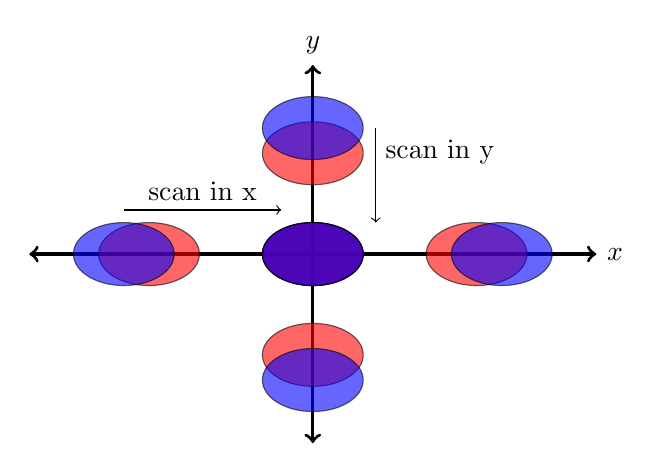
\begin{tikzpicture}[x=.5cm,y=.5cm, scale=1.6]

\draw[<->,very thick] (-4.5,0) -- (4.5,0)node[right] {$x$};
\draw[<->,very thick] (0,-3) -- (0,3) node[above] {$ y$};

%%%%%%%%%%%%%%%%%%%%%%%%%%%%%%%%%%%%%%%%%%%%%%%%%%%%%%%%%%%%%%%%%%%%%%%%%%%%%%%%%

\draw[fill=red, opacity=0.6] (0,-1.6) ellipse (4 mm and 2.5 mm);
\draw[fill=blue, opacity=0.6] (0,-2) ellipse (4 mm and 2.5 mm);


\draw[fill=red, opacity=0.6] (0,0) ellipse (4 mm and 2.5 mm);
\draw[fill=blue, opacity=0.6] (0,0) ellipse (4 mm and 2.5 mm);



\draw[fill=red, opacity=0.6] (0,1.6) ellipse (4 mm and 2.5 mm);
\draw[fill=blue, opacity=0.6] (0,2) ellipse (4 mm and 2.5 mm);


%%%%%%%%%%%%%%%%%%%%%%%%%%%%%%%%%%%%%%%%%%%%%%%%%%%%%%%%%%%%%%%%%%%%%%%%%%%
\draw[fill=red, opacity=0.6] (-2.6,0) ellipse (4 mm and 2.5 mm);
\draw[fill=blue, opacity=0.6] (-3,0) ellipse (4 mm and 2.5 mm);




\draw[fill=red, opacity=0.6] (0,0) ellipse (4 mm and 2.5 mm);
\draw[fill=blue, opacity=0.6] (0,0) ellipse (4 mm and 2.5 mm);



\draw[fill=red, opacity=0.6] (2.6,0) ellipse (4 mm and 2.5 mm);
\draw[fill=blue, opacity=0.6] (3,0) ellipse (4 mm and 2.5 mm);
%%%%%%%%%%%%%%%%%%%%%%%%%%%%%%%%%%%%%%%%%%%%%%%%%%%%%%%%%%%%%%%%%%%%%%%%%%%%%%%%%%%%%%%%%%%%%%
\draw[->,]  (1,2) -- (1,0.5)node[pos=0.25, right] {\text {scan in y}};
\draw[->,]  (-3,.7) -- (-0.5,.7)node[pos=0.5, above] {\text {scan in x}};
\end{tikzpicture}
\end{minipage}
%%%%%%%%%%%%%%%%%%%%%%%%%%%%%%%%%%%%%%%%%%%%%%%%%%%%%%%%%%%%%%%%%%%%%%%%%%%%%%%%%%%%%%%%%%%%%%%%%%%%%%%%%%%%%%%%%%%%%%%%%%%%%%%%%%%%%%%%%%%%%%%%%%%%%%%%%%%%%%%%%
\begin{minipage}[b]{0.5\linewidth}
\centering
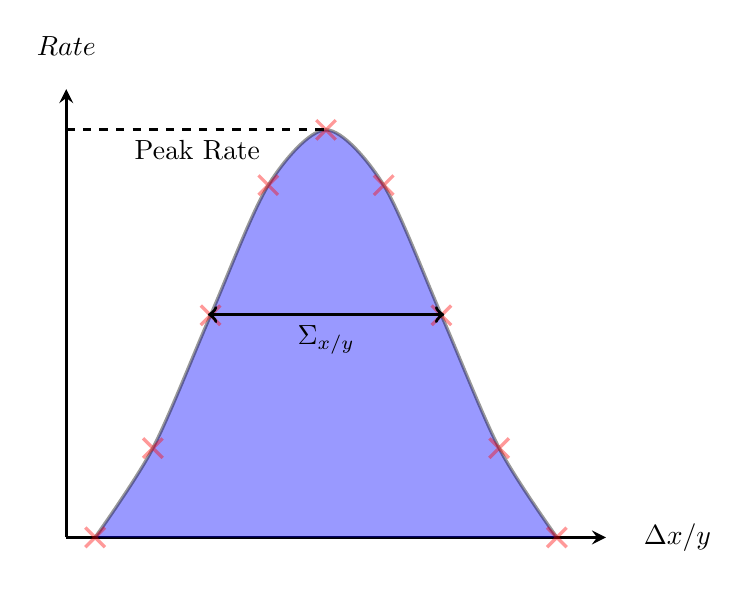
\begin{tikzpicture}
\begin{axis}[every axis plot post/.append style={ color=black,
  mark=x ,domain=-4:4,samples=9,smooth,fill=blue,opacity=0.4, mark size=5pt,mark options={color=red}}, % All plots: from -2:2, 50 samples, smooth, no marks
axis x  line=bottom,very thick, % no box around the plot, only x and y axis
axis y line=left,very thick, % the * suppresses the arrow tips
enlargelimits=upper, xmin=-4.5,
xlabel=\(\Delta x/y\),
ylabel=\(Rate\),
ytick={5},xtick={5},
every axis y label/.style={
    at={(ticklabel* cs:1.05)},
    anchor=south,
},
every axis x label/.style={
    at={(ticklabel* cs:1.05)},
    anchor=west,
},] % extend the axes a bit to the right and top
\addplot[]  {\gauss{0}{2}};


\end{axis}
\draw[<->,very thick] (1.8,2.83) -- (4.8,2.83)node[pos=0.5,below] {$\Sigma_{x/y}$};
\draw[dashed,very thick] (0,5.18) -- (3.33,5.18)node[pos=0.5,below] {\text {Peak Rate}};
\end{tikzpicture}

\end{minipage}
\caption[vdM scan process.]{\textit{Left}: A diagram that shows how the two beams are scanned across the x and y axis. \textit{ Right}: An example of a Gaussian-like function (Blue), being fitted to the rate measurements (red xs) taken during a VDM scan.}
\label{vdm1}
\end{figure}


%%%%%%%%%%%%%%%%%%%%%%%%%%%%%%%%%%%%%%%%%%%%%%%%%%%%%%%%%%%%%%%%%%%%%%%%%%%%%%%%
\section{2018 Calibration Scan program}
The VdM scans, and other scans regarding to calibrations, were performed during the LHC fill 6868 on June 30 and July 1, 2018 at $\sqrt{s}=13TeV$. The LHC filling scheme used 124 colliding bunch pairs at the CMS interaction point (IP5) widely spread over the orbit to reduce long range beam-beam effects and detector afterglow. The resulting beam size $\sigma_{b}$ at the beginning of the fill was in the range of approximately 85–95 and 80–90 $\mu m$ in $x$ and $y$, respectively, increasing over time in the $x$ dimension and decreasing over time in the $y$ dimension.No crossing angle was used for collisions at ATLAS and CMS. The resulting peak pileup was approximately $\mu = 0.6$ , much lower than in a regular physics fill.

The bunch intensities were approximately $7-9 \times 10^{10} $ protons per filled bunch, resulting in a total beam intensity of slightly above $10^{13}$ protons per beam. The total beam intensities were measured with the DC Current Transformers (DCCT) [15], and the bunch currents were measured with the Fast Beam Current Transformers (FBCT) [16]. The beam orbit was monitored using two systems, the DOROS beam position monitors (BPMs) [17] located near IP5, and the arcBPMs located in the LHC arcs adjacent to CMS.  ***The orbit is also tracked using movements of the luminous region based on reconstructed vertices. The arc BPM measurements are translated to a beam position at IP5 using the LHC optics file; the specific optics file used for this scan is R2016c A19mC19mA19mL24.

To ensure a dataset with a high event count for PCC even at large beam separations, CMS recorded the zero-bias triggers on 5 bunch pairs (BCIDs 265, 865, 1780, 2192, and 3380) and recorded events with a total rate of $27.7kHz$.

The CMS VdM scan program was conducted in two parts (``takes''), due to an alarm. The first part consisted of a total of six x-y scan pairs. Two (``emit1'' and ``emit'') were short ``emittance'' scans, in which the two beams were separated by $4sigma_{b}$ in 9 steps with 10 seconds integration time at each scan point.***
Scan pair ``norm1'' was a standard VdM scan, in which the two beams were separated by $6\sigma_{b} \approx 600 \mu m$  and scanned across one another in a sequence of 25 steps with 30 seconds per step.

The second part of the scan program was conducted in the same fill but about $7.5$ hours later. It consisted of twelve scan pairs. Scan pair ``emit3'' was a short emittance scan, followed by scan pairs ``imag2'' and ``imag3'' of the beam imaging kind, an offset scan pair ``offset2'', and finally two normal VdM scan pairs ``norm2'' and ``norm3''. The latter two allow us to test the reproducibility of the measuremen.

****After ``norm3'' scan pair, there were the first superseparation period, in which the beams are separated a distance of $6 \sigma_{b}$ in both $x$ and $y1 direction$ for $5$ minutes long in order to get a bakcground estimation.**** source: Analyis Note 2018


A length scale calibration (LSC) was performed after scan pair ``norm3'' using two different methods. The first, ``lsc1'', was the ``constant separation'' scan, in which the two beams were separated by $1.4\sigma_{b}$ (approximately equal to $1\Sigma$) and moved together in steps of $1\sigma_{b}$ across and back, for a total of $10$ steps with $70$ seconds per step, once in each transverse direction. A second ``variable separation'' method with scan pair ``lsc2'' was also executed, in which one beam (starting with beam 1) is moved to $-2.5\sigma_{b}$ and then a three-point scan (a ``miniscan'') is performed with the other beam (starting with beam 2) at a relative position of $-1.25\sigma_{b}$, $0$, and $+ 1.25 \sigma_{b}$. The position of the first beam is then translated in five steps in the same direction to $+2.5 \sigma_{b}$, repeating the miniscan at each step. This procedure is repeated four times, with two directions for each of the two beams. Each scan point has a duration of about $46s$.

Finally, a normal VdM scan pair “norm4”,*** a second super separation period***,  and two short emittance scan pairs “emit4” and“emit5” concluded the program.


In each scan pair, the scan was performed first in the x direction and then in the y direction, with the exception of the variable separation length scale calibration scan pairs, which were done the other way around.
Figure \ref{2018sp} shows the beam positions for the two beams in the x and y directions as measured by the DOROS BPMs during the scan program, showing all 18 scan pairs.
\begin{center}
    \begin{figure}[H]
        \centering
        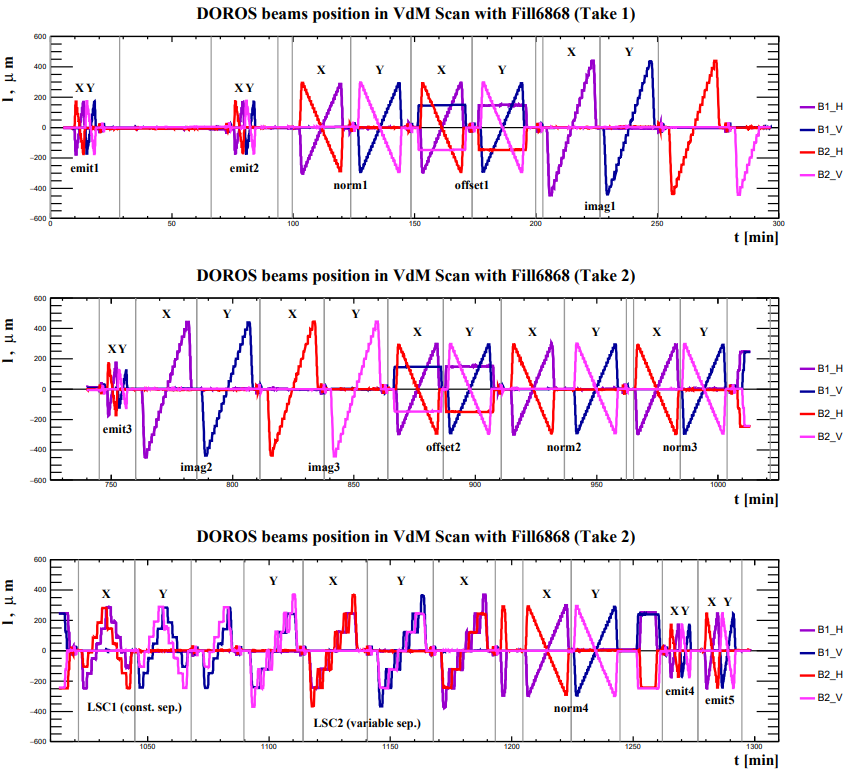
\includegraphics[scale=0.5]{Chapter3/2018Scanprogram.png}
        \caption[2018 San program.]{Relative change in beam positions measured by the DOROS BPMs during the 2018 scan program for the two individual beams in the horizontal x and vertical y planes, as a function of the elapsed time from the beginning of the program. The top row shows the portion ofthe scan program before the alarm at CMS, while the bottom two rows show the scan program after the alarm.[source: pas-lum-18]}
        \label{2018sp}
    \end{figure}
\end{center}

The beam imaging and offset scans are intended for specific studies on the beam shapes described in Section 4**, and they can also be analyzed as traditional van der Meer scans. Both the LSC and beam imaging scans are discussed in detail in Ref. [18**]. The offset scan data is analyzed for the first time in 2018.

source: pas-lum-18
%%%%%%%%%%%%%%%%%%%%%%%%%%%%%%%%%%%%%%%%%%%%%%%%%%%%%%%%%%%%%%%%%%%%%%%%%%%%%%%%%%%%%%%%%%%%%%%%%%%%%%%%%%%%%%%%%%%%%%%%%%%%%%%%%%%%%%%%

\section{Corrections and systematic uncertainties}
There are several systematic effects which affect the beam overlap width measurement, and hence the $\sigma_{vis}$ is extracted from the VdM scan procedure. These effects are measured and, where applicable, corrected as described below, and a systematic uncertainty is assigned to the resulting measured cross section for each source.

Framework correction flags

\begin{itemize}
 \item ghost and satellite
 \item Background (several types, in our case from SS)
 \item Orbit drift (sep and rate)
 \item Beam Beam
 \item DynamicBeta
 \item Length Scale
 \item PeakToPeak
\end{itemize}


%%%%%%%%%%%%%%%%%%%%%%%%%%%%%%%%%%%%%%%%%%%%%%%%%%%%%%%%%%%%%%%%%%%%%%%%%%%%%%%%%%%%%%%%%%%%%%%%%%%%%%%%%%%%%%%%%%%%%%%%%%%%%%%%%%%%%%%%%%%%%%%%%%%

\subsection{Beam beam correction}
Beam beam correction:


\subsection{Veto module correction?}


%%%%%%%%%%%%%%%%%%%%%%%%%%%%%%%%%%%%%%%%%%%%%%%%%%%%%%%%%%%%%%%%%%%%%%%%%%%%%%%%%%%%%%%%%%%%%%%%%%%%%%%%%%%%%%%%%%%

